\section{Introduction}
\label{sec:intro}

% Source: outputs/illustrations/gastroscopy_sequence_warm_final_no_labels/
%         case_0173_gaussian_clusters.pdf (copied without changing the artwork).
% The accompanying selection.json marks the coordinates as schematic_only;
% they are not measured endoscopic spatial coordinates or ACPE outputs.
% Shared caption: English in main.tex; English and Chinese in draft.tex.
\begin{figure}[t]
    \centering
    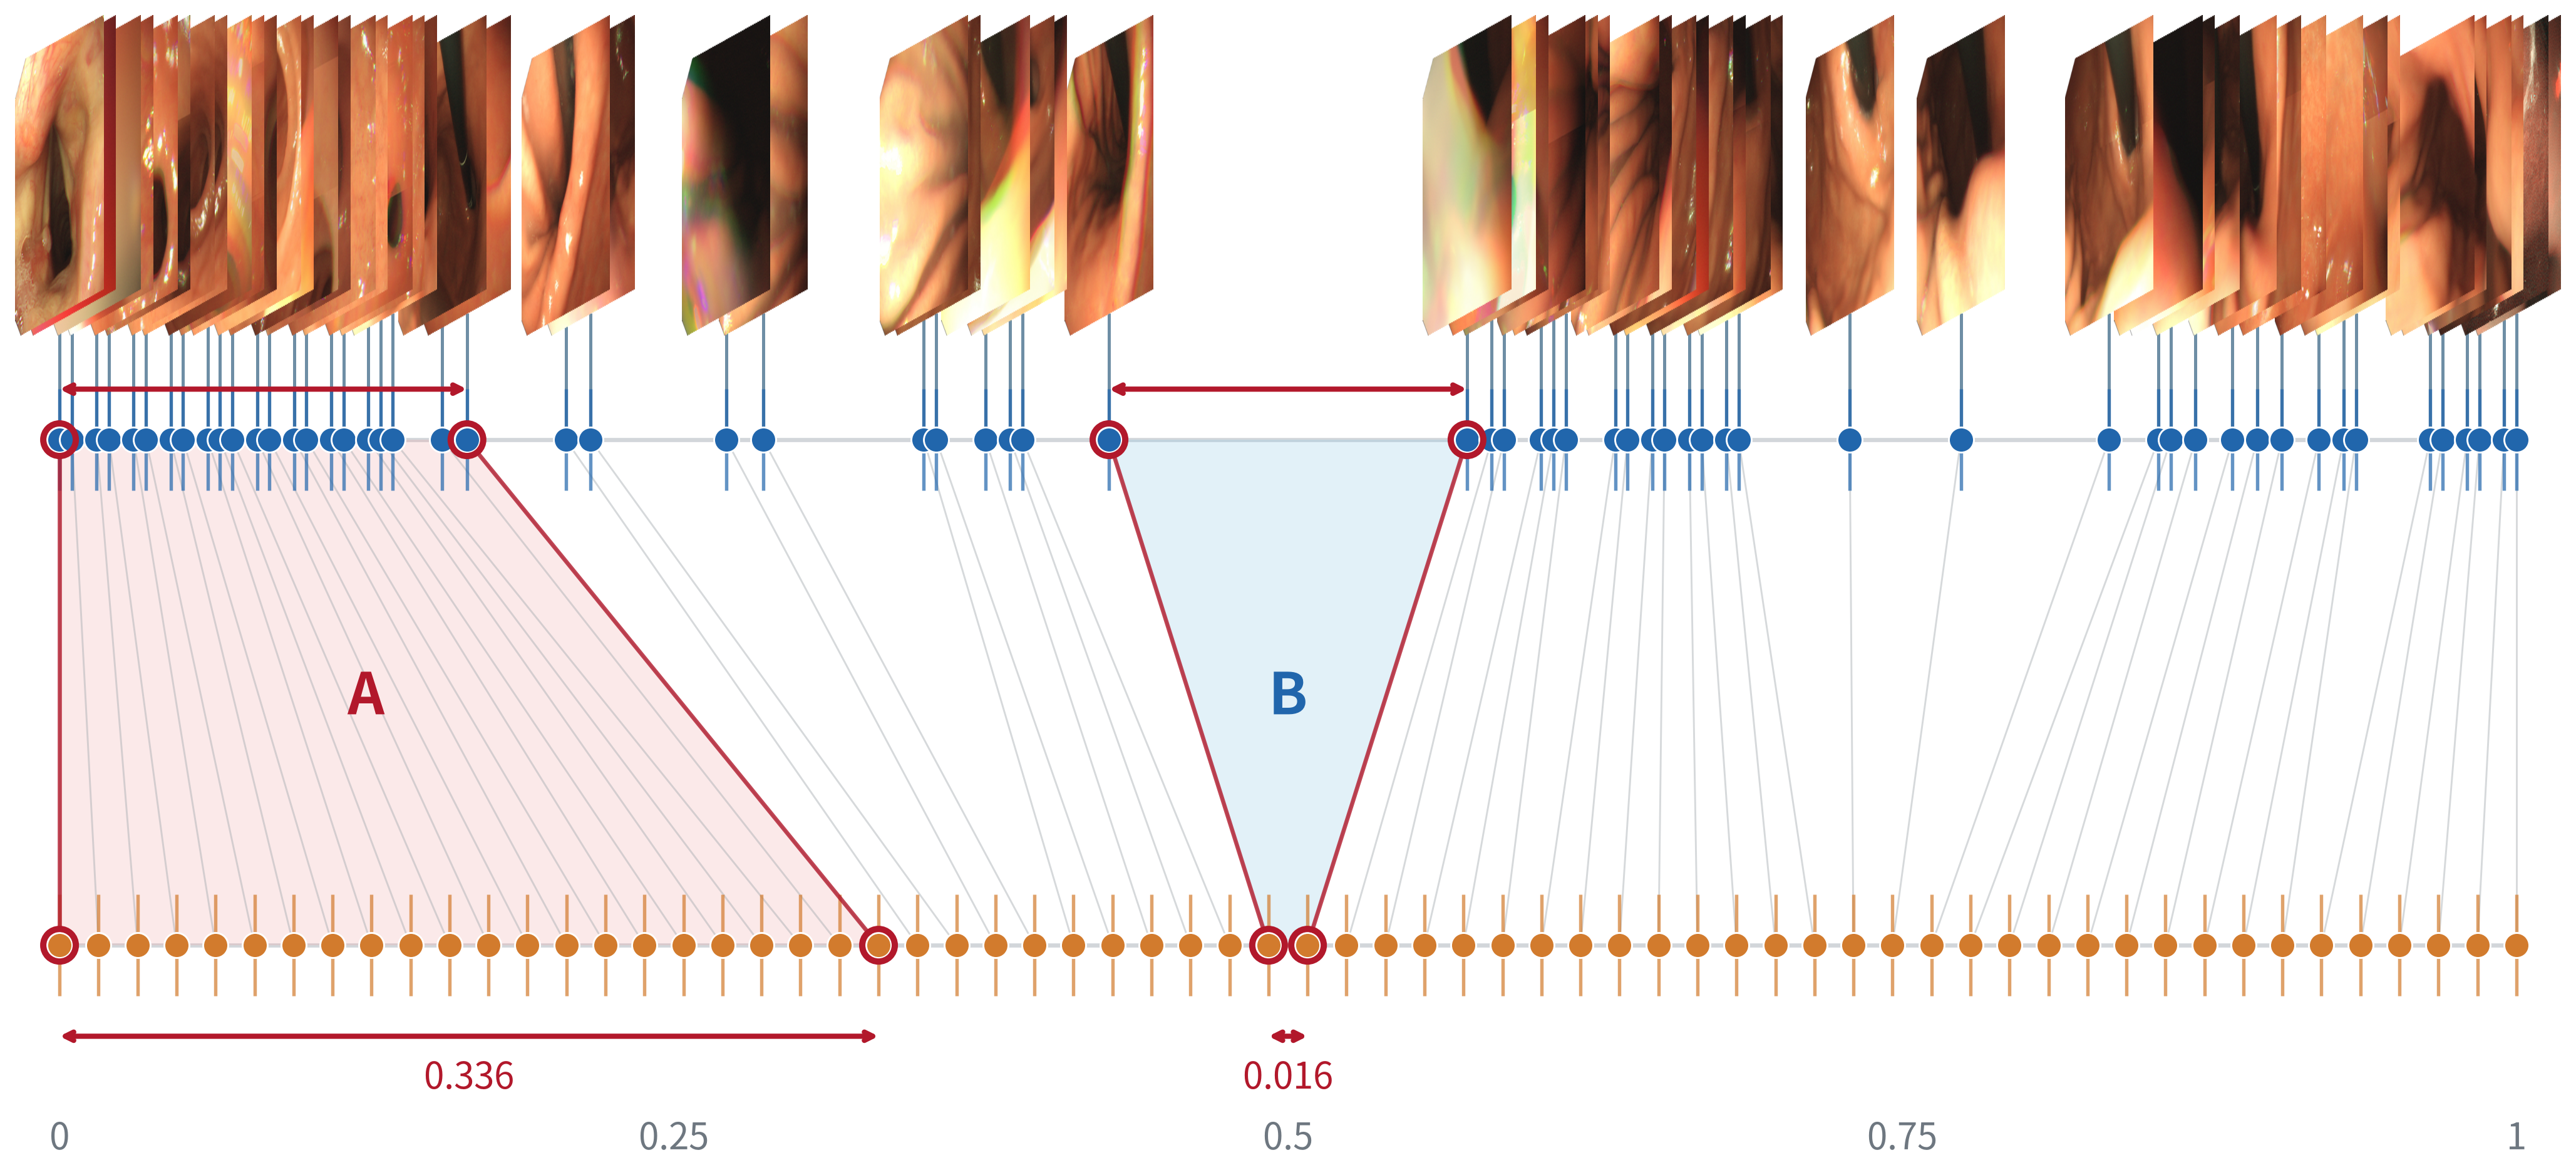
\includegraphics[width=\linewidth]{fig/figure1.pdf}
    \caption[Positional-reference mismatch in discrete examination images.]{%
        Illustration of positional-reference mismatch in discrete examination images.
        Blue and orange nodes show schematic spatial positions and uniformly spaced positional encoding (PE) coordinates, respectively; gray lines connect corresponding images.
        Equal index spacing expands a densely sampled spatial interval (A) and compresses a large gap between consecutive samples (B), distorting inter-image positional relationships.
        Numerical annotations denote normalized PE intervals.
        \cntranslation{%
            离散检查图像的位置参照错配示意图。蓝色与橙色节点分别表示示意性空间位置和等距位置编码（PE）坐标，灰色连线连接对应图像。等距索引将密集采样区间的空间跨度拉大（A），并将相邻采样图像间较大的空间间隔压缩（B），从而扭曲图像间的位置关系。数值标注表示归一化的 PE 间距。
        }%
    }
    \label{fig:position_mismatch}
\end{figure}


% Author-provided introduction; preserve the supplied English and Chinese wording.
% References updated for the current introduction; see refer/intro_citation_notes.md.
% Author claims and experiment summaries remain subject to the new evidence.

In clinical diagnosis, a single examination, such as gastrointestinal endoscopy, may reveal multiple abnormalities, requiring a joint assessment of findings across multiple medical images and the accompanying report. Examination-level multimodal multi-label classification treats each examination as a unified unit of analysis, jointly modeling multiple images and a single paired report to identify abnormalities through complementary visual and textual evidence and support comprehensive clinical assessment. However, existing methods often encode sampled images in an ordered sequence at equally spaced positions, which may not accurately reflect their positional relationships in the actual acquisition setting. Moreover, the report is paired with the examination as a whole, whereas different labels may rely on different images and report passages. Conventional global fusion can obscure these distinctions by combining evidence into a shared representation. These limitations weaken visual context modeling and label-specific evidence integration, hindering reliable recognition of coexisting categories.

\cntranslation{%
在临床诊断中，一次检查（如胃肠内镜检查）可能发现多种异常，需要结合多张医学图像中的异常表现与配套报告进行综合判断。检查级多模态多标签分类以整次检查为分析单元，联合建模多张图像及其配对的一份报告，通过整合互补的视觉与文本证据识别异常，为全面的临床评估提供支持。然而，现有算法常将采样的有序图像按等距位置编码，可能无法准确反映它们在实际采集场景中的位置关系。此外，报告与整次检查整体配对，而不同标签可能依赖不同图像及报告片段中的证据。常规的全局融合将这些证据汇总为共享表征，可能模糊不同标签所需证据之间的区别。这些局限制约了视觉上下文建模与标签特异性证据的整合，进而影响多个共存类别的可靠识别。
}

Unlike video sequences with temporal references or volumetric imaging data with spatial-coordinate metadata, such as computed tomography (CT) and magnetic resonance imaging (MRI), endoscopic snapshots are selectively saved by clinicians during examinations, with acquisition order serving as the only available positional reference. While positional modeling for such discrete examination sequences remains underexplored, related methods for general sequence modeling broadly follow two directions: index-driven encoding and content-adaptive modeling. Index-driven methods refine how supplied positional indices influence attention through improved positional transformations. ComRoPE~\cite{yu2025comrope} introduces trainable commuting angle matrices to improve rotary position encoding, while VideoRoPE~\cite{wei2025videorope} incorporates temporal allocation and adjustable spacing to represent spatiotemporal structure. However, these positional mappings do not explicitly adapt to visual similarities between images in the current sequence. To incorporate content-dependent contextual cues, content-adaptive methods introduce input-dependent mechanisms into positional or attention modeling: PaTH~\cite{yang2025path} accumulates input-dependent Householder transformations, while DAPE V2~\cite{zheng2025dapev2} processes attention scores across neighboring positions and attention heads. Overall, these approaches enhance sequence modeling through index-based positional transformations or content-dependent adjustments to token interactions.

\cntranslation{%
不同于具有时间参照的视频序列，以及计算机断层扫描（CT）和磁共振成像（MRI）等具有空间坐标信息的三维影像数据，内镜图像由医生在检查过程中选择性手动保存，采集顺序是唯一可用的位置参照。针对这类离散检查序列的位置建模研究仍然有限，现有通用序列位置建模方法主要沿两类思路展开：索引驱动编码与内容自适应建模。索引驱动方法以给定的位置索引为基础，通过改进位置变换调节位置信息对注意力交互的影响。ComRoPE~\cite{yu2025comrope} 引入可学习的可交换角度矩阵，增强旋转位置编码的表达能力；VideoRoPE~\cite{wei2025videorope} 则通过时间维度分配与可调间距表达时空结构。然而，这类位置映射并未显式根据当前序列中图像之间的视觉相似性进行自适应调整。为引入内容相关的上下文线索，内容自适应方法将输入相关的机制融入位置或注意力建模：PaTH~\cite{yang2025path} 累积由输入决定的 Householder 变换，DAPE V2~\cite{zheng2025dapev2} 则联合处理相邻位置与不同注意力头的注意力分数。总体而言，这些方法通过基于索引的位置变换或内容相关的 token 交互调整，增强序列建模能力。
}

Beyond multi-image sequence modeling, examination-level multimodal multi-label recognition requires integrating an image collection with its paired report while distinguishing the evidence supporting different coexisting labels. Related studies provide complementary approaches through cross-modal interaction and label-aware representation learning. SAIF~\cite{zhang2025saif} aligns image–text features and selects correlated features before attention-based fusion, while MMTF~\cite{zhong2026mmtf} combines token exchange with multiscale cross-attention to integrate image and report representations. For multi-label recognition, MambaML~\cite{zhu2025mambaml} aggregates visual information into label embeddings and models label dependencies to obtain label-specific representations. Wang et al.~\cite{wang2025granularity} further enrich class representations with structured textual descriptions and align their semantics within a shared image–text embedding space. Overall, these studies improve recognition by strengthening cross-modal information exchange and incorporating label-specific semantics into representation learning.

\cntranslation{%
除了多图像序列建模，检查级多模态多标签识别还需要整合整个图像集合及其配对报告，并区分支持不同共存标签的证据。 相关研究通过跨模态交互与标签感知表征学习提供了互补的处理思路。SAIF~\cite{zhang2025saif} 对齐图文特征，并在注意力融合前筛选具有较强相关性的特征； MMTF~\cite{zhong2026mmtf} 则结合 token 交换与多尺度交叉注意力，整合图像与报告表征。 针对多标签识别，MambaML~\cite{zhu2025mambaml} 将视觉信息聚合至标签嵌入，并建模标签依赖关系，形成标签特异性表征。 Wang 等人~\cite{wang2025granularity}进一步利用结构化文本描述丰富类别表征，并在共享图文嵌入空间中对齐其语义。 总体而言，这些研究通过增强跨模态信息交互，以及将标签特异性语义引入表征学习，改善识别能力。
}

Despite these advances in positional modeling and cross-modal interaction, important limitations remain. First, distances between sampled indices do not necessarily reflect actual spatial relationships: spatially adjacent images may be assigned widely separated positions, whereas spatially distant images may be assigned overly close positions, as illustrated in Fig.~\ref{fig:position_mismatch}. Index-driven methods improve the encoding of these indices but still describe inter-image positional relationships through index distances. Content-adaptive methods incorporate visual information into positional modeling; however, if they retain distorted index distances as their reference, their adjustments change how positional information is used rather than correcting the positional reference itself. The original spacing mismatch may therefore persist in subsequent modeling. Thus, an important modeling challenge is to reconstruct positional references from visual changes while preserving acquisition structure, so that contextual intervals are no longer determined solely by fixed indices. Second, examination-level pairing associates an entire image collection with one report without specifying which images and report passages support each coexisting label. Global fusion can blur these distinctions within a shared representation, while label-aware visual modeling or class-level semantic alignment alone does not establish correspondence with relevant passages in the examination-specific report. Moreover, the relevance of textual evidence varies across labels and examinations, requiring different contributions to individual predictions. Without consistently organizing visual aggregation, label interactions, textual retrieval, and fusion around each label, multimodal modeling may mix unrelated evidence and fail to exploit complementary information selectively.

\cntranslation{%
尽管上述方法增强了位置建模与跨模态交互，但仍存在关键局限。首先，采样索引之间的距离并不一定反映实际空间关系：实际邻近的图像可能被编码得过远，而实际相距较远的图像却可能被编码得过近，如图~\ref{fig:position_mismatch}~所示。索引驱动方法改进了这些索引的编码方式，却仍依据索引间距描述图像的位置关系。内容自适应方法虽引入图像信息优化位置相关建模，但若仍沿用存在偏差的索引间距作为参照，其调整改变的只是模型如何使用位置信息，而不是纠正位置参照本身，原有的间距偏差因而仍可能影响后续建模。因此，如何在保留采集结构的同时，利用视觉变化重新构建位置参照，使上下文间距不再仅由固定索引决定，仍是一个重要的建模问题。 其次，检查级配对将整个图像集合与一份报告关联起来，却未明确哪些图像及报告片段支持各个共存标签。全局融合可能在共享表征中模糊这些区别，而仅进行标签感知的视觉建模或类别级语义对齐，也未建立与当前检查报告中相关片段的对应关系。此外，文本证据的相关性会随标签和检查样本变化，因此需要对各个预测提供不同程度的支持。如果视觉聚合、标签交互、文本检索与融合未能始终围绕各个标签进行组织，多模态建模就可能混合无关证据，难以有选择地利用互补信息。
}

To this end, we develop Acquisition-aware Label-centric Multimodal Multiple Instance Learning (ALM-MIL), an examination-level multimodal multi-label framework built upon Acquisition-aware Contextual Position Encoding (ACPE) and Label-Centric Coexistence Fusion (LCCF). ACPE anchors sampled images to their original acquisition coordinates and constructs content-adaptive contextual positions according to visual transitions, while preserving the monotonic structure of the acquisition sequence. In this way, the positional relationships among sampled observations are no longer restricted to uniformly spaced representations. LCCF further organizes multimodal evidence around individual labels. Specifically, it first aggregates label-specific visual evidence, models higher-order interactions among coexisting labels through hypergraph reasoning, retrieves label-relevant textual evidence from the paired report, and finally adaptively controls its contribution through label-wise gated fusion. Together, ACPE and LCCF enable the model to better represent acquisition relationships among multiple images while aligning examination-level image–report information with label-level prediction. Extensive experiments across private clinical cohorts and public datasets demonstrate the effectiveness and generalizability of ALM-MIL.

\cntranslation{%
为此，我们构建了采集感知的标签中心多模态多实例学习框架（Acquisition-aware Label-centric Multimodal Multiple Instance Learning，ALM-MIL），用于检查级多模态多标签分类，其核心由采集感知上下文位置编码（Acquisition-aware Contextual Position Encoding，ACPE）和标签中心共存融合（Label-Centric Coexistence Fusion，LCCF）组成。ACPE 以采样图像的原始采集坐标为锚点，并根据图像之间的视觉变化构建内容自适应的上下文位置，同时保持采集序列的单调结构，从而使采样观测之间的位置关系不再局限于规则等距表示。LCCF 则进一步围绕各个标签组织多模态证据。具体而言，它首先聚合标签特异性的视觉证据，通过超图推理建模共存标签之间的高阶关系，随后从配对报告中检索与各标签相关的文本证据，并通过标签级门控融合自适应控制其贡献。ACPE 与 LCCF 的结合，使模型既能够更准确地表达多张图像之间的采集关系，又能够将检查级图文信息与标签级预测进行对应。我们在多个私有临床队列和公开数据集上的大量实验验证了 ALM-MIL 的有效性与泛化能力。
}

Our main contributions are summarized as follows:

\cntranslation{%
本文的主要贡献总结如下：
}

\begin{itemize}
    \item We identify and investigate the mismatch between sampling-index distances and actual spatial relationships in discrete examination images. This perspective shifts attention from improving the encoding of supplied indices to examining the validity of the positional reference itself.

    \cntranslation{%
    我们指出并研究离散检查图像中，采样索引距离与实际空间关系之间的错配问题。 这一视角将关注点从改进给定索引的编码方式，转向审视位置参照本身的合理性。
    }

    \item We propose ACPE to learn content-adaptive contextual intervals under explicit acquisition-structure constraints, moving beyond fixed index spacing while preserving acquisition order and the overall sequence span.

    \cntranslation{%
    我们提出 ACPE，在显式采集结构约束下学习内容自适应的上下文间距，突破固定索引间距的限制，同时保持采集顺序与整体序列跨度。
    }

    \item We develop LCCF, a pipeline specifically designed for multimodal multi-label classification using multiple examination images and a single paired report. By organizing visual and textual evidence around individual labels, LCCF offers a more targeted alternative to generic fusion pipelines for recognizing coexisting abnormalities.

    \cntranslation{%
    我们提出 LCCF，专门面向多张检查图像与一份报告配对的多模态多标签共存分类任务。LCCF 围绕各个标签组织视觉与文本证据，相比通用融合流程，更有针对性地满足共存异常识别中不同标签的证据需求。
    }

    \item We evaluate ALM-MIL on real-world clinical cohorts and public datasets, examining classification performance, robustness to missing images, and the contributions of individual designs.

    \cntranslation{%
    我们在真实临床队列与公开数据集上评估 ALM-MIL，考察其分类性能、图像缺失鲁棒性及各项设计的贡献。
    }

\end{itemize}
